\documentclass[master]{exam} 
\usepackage{fullpage}
\usepackage{amsmath}
\usepackage{comment}
\usepackage{graphicx}

\begin{document}

\examheader{CISC 106}{UEF Example}{Developed: 2010}

\section{Topic}

\begin{block}{FSA Description}
  In the following four problems, let $A$ denote a finite-state
  automaton with exactly one accepting state.
\end{block}

\begin{problem}{topic}{15}
  This is a problem
  \begin{answers}
    \answer[correct] correct answer 1
    \answer answer 2
    \answer[fixed] fixed answer 3
    \answer[correct,fixed] correct fixed answer 4
    \answer answer 5
    \answer[fixed,correct] fixed correct answer 6
  \end{answers}
\end{problem}

\begin{problem}{Arithmetic}{5}
  \label{prob:arithmetic:prime}
  Which of the following is not prime?
  \begin{answers}
    \answer[correct] $2^{-1}$
    \answer[correct] $2^0$
    \answer $2^1$
    \answer $3^1$
    \answer[fixed] none of the above
  \end{answers}
\end{problem}

\begin{figure}[placement h]
  \begin{center}
      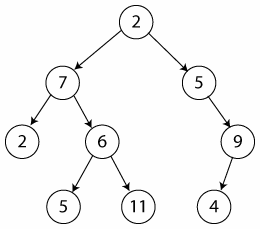
\includegraphics[scale=0.50]{binary_tree.png}
      \caption{Traverse Binary Tree}
      \label{fig:binary tree}
   \end{center}
\end{figure}

\begin{block}{Goodbye Message}
  Did you remember to write your name on the first page?  Did you
  attempt to answer every question?    Have a good holiday.
\end{block}

\end{document}







